\chapter{Asking Supercar Owners How They Got RICH! (Florida)}

We begin, as the lecture begins, with spectacle: luxury cars, clipped income figures, lawsuits, sales lines, and the promise that visible wealth will be translated into usable rules. The point of the chapter is not to glorify the cars. It is to follow the order in which the lecture turns those cars into evidence. Again and again the host asks the same questions: What is the asset? What is the business? How long has the business been running? What is the largest single-year outcome? Only after that does he ask for mechanism. In this way the lecture builds a small quantitative theory of entrepreneurship out of field interviews rather than abstractions.

\section{Preview, Tampa, and the Problem of Visible Wealth}

The opening montage is a preview, not yet the main line of argument. It flashes future claims before we know who is speaking: a healthcare entrepreneur, a hedge-fund owner, a lobbyist and publicist, several annual earning figures, and at least one story of litigation by large corporations. The lecture uses this preview exactly as a lecturer might use a list of coming results: it tells us what kind of objects will matter before it tells us why.

Only after that preview does the host state the field problem. Tampa is presented as a city dense with wealth, and the host's explicit aim is to ask multimillionaires and business owners how they became wealthy and how a viewer might begin a path toward financial freedom. The governing city-level claim is
\begin{equation}
N_{\text{millionaires}}(\text{Tampa}) > 50{,}000.
\end{equation}
We should keep this as a framing claim made inside the lecture, not as an independently established demographic theorem. Its role is methodological: the city is treated as a sample space rich in entrepreneurial cases.

\begin{table}
\centering
\begin{tabular}{|l|l|l|l|}
\hline
Interviewee & Business & Time in Business & Peak Single-Year Result \\
\hline
Healthcare entrepreneur & medical sleep testing & $\approx 28$ years & multiple eight figures \\
Digital-asset operator & hedge fund & $\approx 10$--$11$ years & $\$4.5\,\mathrm{M}$ \\
Entrepreneur since 2019 & unspecified business & since 2019 & $\$2.5\,\mathrm{M}$ \\
Lobbyist/publicist & consulting practice & $\approx 15$ years & $\$1.4\,\mathrm{M}$ \\
\hline
\end{tabular}
\caption{The four principal cases as they are introduced in the lecture.}
\end{table}

This opening table is already enough to show the lecture's structure. We are not moving through one continuous doctrine. We are moving through four local models, stitched together by recurring prompts and recaps.

\section{The Healthcare Entrepreneur: Advice Filters, Low Liquidity, and the Competitive Frontier}

After the preview, the lecture returns to the first sustained case. The speaker identifies himself as a healthcare entrepreneur and says he owns the largest medical sleep testing company in the United States. He places himself on a long business horizon,
\begin{equation}
t_{\text{biz,health}} \approx 28\ \text{years},
\end{equation}
and describes his best single year only loosely as ``multiple eight figures.'' The looseness matters. We are meant to hear magnitude, not a finely audited line item.

The host then asks for the best financial advice he has received, and the lecture's first clean decision rule appears. The speaker's claim is domain-specific: do not take money advice from people who make less money than you; do not take business advice from people with smaller businesses; do not take relationship advice from people with failed marriages; and, in the garbled friendship line, do not take advice about friendship from people who do not sustain it.

\begin{definition}
Let
\[
d \in \{\text{money},\text{business},\text{relationship},\text{friendship}\}
\]
denote a domain of advice, and let \(O_d(i)\) be the realized outcome of person \(i\) in that domain. A careful reconstruction of the speaker's rule is the \emph{advice filter}: prefer advisor \(i\) to advisor \(j\) only when
\begin{equation}
O_d(i) > O_d(j).
\end{equation}
The inequality is a reconstruction, but it captures the lecture's insistence that authority is local to demonstrated performance.
\end{definition}

The next move is what makes the section pedagogically strong. The speaker does not leave the advice rule in the air. He immediately shifts to a broke point: nine years earlier, he says, he had only \(\$78\) in the bank, and he sharpens this by specifying that \(\$78\) was his \emph{available} balance. That gives us a minimal liquidity equation:
\begin{align}
B_{\text{avail}} &= \text{\$}78,\\
B_{\text{post}} &= B_{\text{avail}} - C_{\text{out}},
\end{align}
where \(C_{\text{out}}\) is the value of outstanding checks or pending obligations. The consequence follows at once:
\begin{equation}
C_{\text{out}} > \text{\$}78
\quad \Rightarrow \quad
B_{\text{post}} < 0.
\end{equation}
The lecture is making a sharp distinction here. One can be poor in a broad emotional sense, but the more urgent entrepreneurial fact is operational fragility. If the buffer is thin enough, routine obligations can become catastrophic.

\paragraph{Worked example.}
Suppose a pending check clears in the amount of \(\$100\). Then
\begin{equation}
B_{\text{post}} = \text{\$}78 - \text{\$}100 = -\text{\$}22.
\end{equation}
Nothing sophisticated is happening in the arithmetic, but the lecture's point is not arithmetic virtuosity. It is that near-zero liquidity compresses time. A small payment can produce immediate failure.

Only after this broken-balance story does the host ask the next structural question: healthcare is very competitive, so what sets this operator apart from most of the field? The answer is the lecture's first explicit market model. Competition, says the speaker, is not bad news by itself. It usually means there is money in the arena. The real issue is not how many people enter but how few actually perform at the upper tail. The quantitative claim is given cautiously as
\begin{equation}
p(R > \text{\$}10\,\mathrm{M}) < 0.01.
\end{equation}
The speaker also adds a second number---something like ``\(0.07\)''---but the normalization is unclear, so the safe lesson is only that the upper tail is very small.

A clean transcript-faithful reconstruction is
\begin{equation}
N_{\text{elite}} = p_{\text{elite}}N,
\qquad
p_{\text{elite}} \ll 1,
\end{equation}
where \(N\) is the number of entrants in a market and \(N_{\text{elite}}\) is the genuinely high-performing upper tail. The lecture's rhetoric is rough, but the structure is clear: a market can be crowded at the entrance and sparse at the frontier.

\begin{remark}
The host later summarizes this section by saying the speaker laid out what it takes to become a ``top \(1\%\) entrepreneur.'' That is recap language, not a theorem proved in the interview. We should keep the speaker's own stronger point: crowding and opportunity can coexist because discipline is rare.
\end{remark}

\begin{proposition}
A competitive market may still be open at the frontier.
\end{proposition}

\begin{proof}
Suppose an industry has many participants, so the surface count \(N\) is large. If only a small fraction \(p_{\text{elite}}\) actually sustains the discipline, grind, and execution needed to reach serious scale, then the effective frontier contains only \(N_{\text{elite}} = p_{\text{elite}}N\) real competitors, with \(p_{\text{elite}} \ll 1\). Thus crowding at the level of entry does not imply crowding at the level of elite execution.
\end{proof}

\subsection{Question \& Answer}

\paragraph{Question.} Why does the speaker welcome competition rather than fear it?

\paragraph{Answer.} Because he reads competition as evidence that the market is real and economically meaningful. The deeper variable is not entry volume but frontier scarcity. Most people join a market; far fewer remain in the thin upper tail that truly executes. The lecture's answer is therefore not ``run from crowded industries,'' but ``distinguish the crowd from the frontier.''

\begin{figure}
\centering
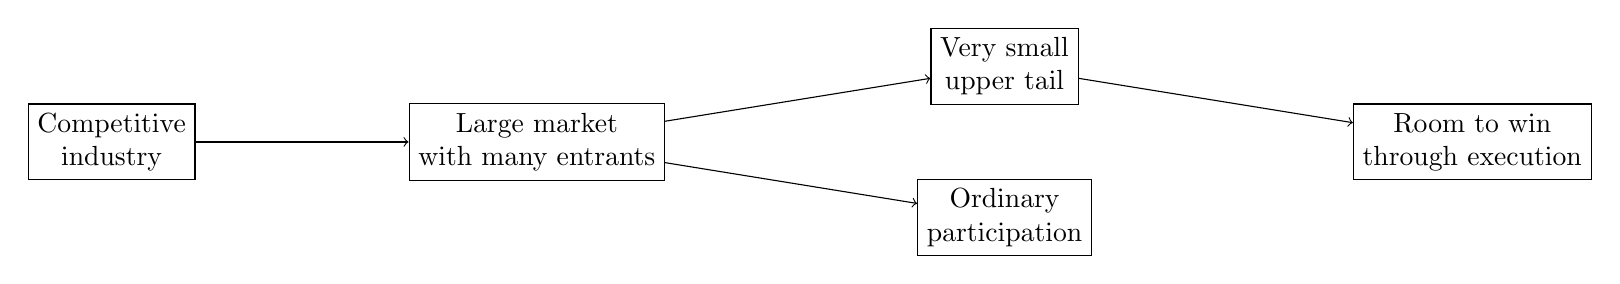
\begin{tikzpicture}[x=2.7cm,y=1.2cm]
\node[draw,rectangle,align=center] (a) at (0,0) {Competitive\\industry};
\node[draw,rectangle,align=center] (b) at (2.0,0) {Large market\\with many entrants};
\node[draw,rectangle,align=center] (c) at (4.2,0.8) {Very small\\upper tail};
\node[draw,rectangle,align=center] (d) at (4.2,-0.8) {Ordinary\\participation};
\node[draw,rectangle,align=center] (e) at (6.4,0) {Room to win\\through execution};
\draw[->] (a) -- (b);
\draw[->] (b) -- (c);
\draw[->] (b) -- (d);
\draw[->] (c) -- (e);
\end{tikzpicture}
\caption{A transcript-derived schematic of the first interview's market argument.}
\end{figure}

The host's recap is worth preserving. He does not merely say that the man is rich. He says, in effect, that we have just seen a blueprint: recovery from near-zero liquidity, a willingness to delegate, an emphasis on selling, and the refusal to be intimidated by competitive markets. This is how the lecture itself tells us to read the first case.

\section{The Hedge-Fund Operator: Presupposing the Close and Filtering for Stress Tolerance}

The next major case begins in the same way. Again the asset is a Rolls-Royce; again the speaker is identified by business first. This time the business is a hedge fund for digital assets, with a time horizon of roughly a decade and a peak annual result of
\begin{equation}
R_{\text{peak,hedge}} = \text{\$}4.5\,\mathrm{M}.
\end{equation}
Only then does the host ask for the best sales and negotiation advice.

The answer is compact: assume the close. The speaker immediately explains the phrase. One talks to the other person as though the commercial relationship is already moving forward. He then adds a second ingredient: make the person laugh. The lecture's implicit model is therefore
\begin{equation}
P(\text{close}\mid \text{assume close},\ \text{rapport})
>
P(\text{close}\mid \text{neutral framing},\ \text{low rapport}).
\end{equation}
This is not statistical evidence. It is a practitioner's heuristic. But it is more than a slogan. It says that framing and affect matter. We do not merely pitch; we position the interaction as though the transaction already belongs to the natural future of the conversation.

The lecture then turns sharply. The host asks for the lowest point in the speaker's career, and the answer is a lawsuit involving large corporations and one of his companies. The speaker says he won and says good business insurance covered much of the burden. This shift is important. We are not allowed to stay in the pleasant geometry of sales psychology. The lecture insists that conversion skill and downside exposure coexist.

We may summarize the internal logic of the section as follows:
\begin{enumerate}
\item presuppose movement toward the close;
\item reduce resistance by generating liking;
\item remember that operating businesses are still exposed to legal and contractual shocks;
\item therefore protect the downside as aggressively as one pursues the upside.
\end{enumerate}

The host then asks whether everybody can be an entrepreneur. The answer is flatly negative. The speaker defines the entrepreneurial role as constant problem-fixing under stress and repeated trials. In that sense the lecture tightens the optimism of the first section. A competitive market may be open, yes, but that does not imply universal suitability for the path.

\subsection{Question \& Answer}

\paragraph{Question.} If sales skill and confidence matter so much, why is entrepreneurship still ``not for everybody''?

\paragraph{Answer.} Because the lecture defines entrepreneurship not by desire but by repeated exposure to volatility, legal risk, and unresolved problems. The person who can frame a conversation well may still fail if he cannot carry stress, absorb shocks, and keep solving problems when the conversation is over.

The host's recap after this interview is again a teaching device. He compresses the lesson into blunt public language: this path is not for everybody; it involves trials and tribulations; yet if one is built for it, one must work, reinvest, and stop waiting for mystery. The lecture is careful to keep the glamour of the car attached to the harshness of the process that precedes it.

\section{The Entrepreneur Since 2019: Confidence, Marriage, Faith, and Money Discipline}

At this point the lecture relaxes its tone without relaxing its structure. The next speaker identifies herself simply as an entrepreneur, says she has been in business since \(2019\), and reports a best year of
\begin{align}
R_{\text{peak,woman}} &= \text{\$}2.5\,\mathrm{M},\\
a_{\text{current,woman}} &= 40.
\end{align}
She also says she has been broke several times before and that only recently has she hit her stride. So even here, where the tone becomes gentler, the lecture keeps the collapse-and-rebuild motif in view.

The host asks what advice she would give to her twenty-year-old self. Her answer is belief: believe in yourself. But the lecture does not allow that answer to float as pure interiority. The next question asks how such belief was actually found, and she answers concretely: her husband. He is described as the one who kept telling her to go out, get it, and try. The lesson is that confidence is not merely an inner possession. Often it is stabilized by a nearby person who keeps directing action forward.

This leads immediately to the question of marriage. How important is it to marry the right person? Her answer is again operational rather than sentimental: the wrong person pulls you in the opposite direction from the life you are trying to build. The lecture is still speaking about direction, leverage, and energy flow; it has simply moved those ideas into the domestic sphere.

Then comes faith. She calls faith her backbone, the thing she relies on day by day. And after this interior and relational sequence comes the financial rule: do not overextend yourself, and make sure money works for you rather than against you. A cautious reconstruction of that warning is
\begin{equation}
\text{Overextension} \uparrow
\qquad \text{as} \qquad
\frac{\text{fixed obligations}}{\text{cash flow}} \uparrow.
\end{equation}
The point of the equation is not to impose formalism on a plainspoken line. It is to show the structure buried inside the line. When obligations outrun reliable cash generation, control reverses. One stops directing capital and starts serving it.

This section matters because it widens the lecture's explanatory frame. After competition, sales, and insurance, we are asked to think about support systems, confidence formation, marriage choice, faith, and disciplined financial architecture. The lecture is telling us that business success is not purely a market phenomenon. It is also an arrangement of the self and its immediate world.

\section{The Lobbyist and Publicist: Hunger, Silence, and the Outside Option}

The final major case begins with another status object, but the lecture quickly strips away the surface. The speaker identifies himself as a lobbyist and publicist with a consulting practice, gives a time horizon of roughly fifteen years, and reports
\begin{align}
t_{\text{biz,lobby}} &\approx 15\ \text{years},\\
R_{\text{peak,lobby}} &= \text{\$}1.4\,\mathrm{M}.
\end{align}
He immediately adds the caveat that the following year he almost lost everything while trying to build and scale an agency. This is an important piece of rhythm. The lecture refuses to let a peak-year number stand by itself.

Asked whether he could make it all back if he went broke tomorrow, he says yes, and his reason is hunger. He knows how to live near the floor. He describes choosing between transit and food, enduring low-consumption conditions, and taking hard labor before launching his company. That gives us a resilience model: if the personal floor is low enough, downside loses some of its power to paralyze.

His own timeline is then stated explicitly:
\begin{align}
a_{\text{current,lobby}} &= 38,\\
a_{\text{millionaire,lobby}} &= 35.
\end{align}
Again, the lecture emphasizes build time rather than miracle.

The host next asks for the best advice he ever got from a mentor, and two maxims appear. First: never let them see you sweat. Second: do not believe your own propaganda. The first is public composure under pressure. The second is internal discipline under success. The speaker supports both claims with a long anecdote about making money quietly while continuing to look externally ordinary, precisely to avoid hostility and premature attention. Moving in silence is presented not as mysticism but as social strategy.

The host then returns to sales and asks how this speaker lands large political deals in a competitive arena. The answer is the lecture's cleanest bargaining rule: be able to walk away.

\begin{definition}
The \emph{outside option} \(O_{\text{outside}}\) is the credible value of refusing the present deal and continuing elsewhere. The \emph{bargaining leverage} \(L_{\text{bargain}}\) is the strength one carries into negotiation by virtue of having such an option.
\end{definition}

The transcript-derived leverage relations are
\begin{align}
O_{\text{outside}} \uparrow &\Rightarrow L_{\text{bargain}} \uparrow,\\
\text{Neediness} \uparrow &\Rightarrow L_{\text{bargain}} \downarrow.
\end{align}
The speaker then adds a stronger heuristic: the first person to speak loses. We need not elevate that to a universal theorem. Its role is narrower. It tells us that one should not rush to reveal weakness or desperation. Instead one presents value: consistency, case studies, cadence, and terms. If the buyer wants cheap, let the buyer leave.

\subsection{Question \& Answer}

\paragraph{Question.} What creates leverage in a competitive sales environment?

\paragraph{Answer.} Not noise, and not theatrical confidence by itself. The lecture's answer is a pair: demonstrated value and a credible outside option. One becomes harder to bargain down when one can both prove worth and refuse the deal.

\section{Power, Bureaucracy, and the Final Layer of Belief}

From bargaining the lecture widens to institutions. Asked whether politicians are corrupt, the speaker reframes the matter and says that power corrupts. Asked about the biggest lie we are told by government, he attacks the simple slogan that one can merely ``drain the swamp'' and instead says that bureaucrats and lobbyists often carry the durable technical knowledge of the system. These are his claims, not canonical political theory, and we should preserve that attribution.

Still, the transition is not accidental. The lecture has been moving outward in concentric circles: from personal liquidity, to market competition, to sales technique, to resilience, to social image, and now to public power. The recurring claim is that what governs outcomes is often not what is most visible. Surface politics is not the full machine, just as surface wealth is not the full process.

The final movement is theological. Asked whether he believes in God, the speaker answers in explicitly Christian language and then goes further, describing faith as central to his life and work. In the lecture's sequencing this matters. Theology arrives last, after tactics, pain, leverage, and institutions. It is presented not as an alternative to the previous operating rules but as the deepest layer under them.

The lecture then closes in the expected register of a digital field series: a brief channel lift, a newsletter invitation, and a pointer to the next video. That closing is administrative, but it also tells us something about the genre. These notes belong to an interview-driven entrepreneurial lecture, not to a sealed classroom proof. The argument is extracted from movement through the city.

\section{Summary}

If we keep the lecture in order, its logic is stronger than it first appears. It begins with visible wealth, but it does not stay there. It asks us to translate spectacle into structure. The principal rules are these:
\begin{itemize}
\item use outcome filters when deciding whose advice counts;
\item treat low liquidity as a hard operational equation, not a vague feeling;
\item do not confuse a crowded market with a closed frontier;
\item in sales, presuppose movement and increase liking;
\item protect the downside, because closing deals does not eliminate shocks;
\item admit that entrepreneurship selects for stress tolerance rather than universal desire;
\item understand that confidence is often socially supported rather than purely private;
\item do not overextend, or money will begin to work against the owner;
\item preserve leverage by building a real outside option and a real proof of value.
\end{itemize}

This is why the lecture works as a chapter. The cars are only the opening symbols. The real content is the sequence of local models by which the speakers explain survival, selection, scale, and control.